\documentclass[a4paper, 12pt, titlepage]{article}

\usepackage{amssymb}
\usepackage{amsmath}
\newtheorem{theorem}{Theorem}
\newtheorem{lemma}{Lemma}
\newtheorem{proof}{Proof}

\usepackage[noend]{algpseudocode}
\usepackage{algorithmicx,algorithm}
\renewcommand{\algorithmicrequire}{\textbf{Input:}}
\renewcommand{\algorithmicensure}{\textbf{Output:}}

\usepackage{mathtools}

\usepackage{graphicx}

\usepackage{indentfirst}
\setlength{\parindent}{2em}
\usepackage[CJKbookmarks]{hyperref}

\title{Notes for Min-Cut and Max-Cut}
\author{ritchie huang}
\date{2019-09-20}

\begin{document}

\maketitle 

\tableofcontents
\newpage

\section{Understand Karger's Min-Cut Algorithm}
Let \textbf{G} be the graph with \textbf{n} nodes, \textbf{C} be the min-cut. 

\subsection{Pseudocode for Karger's Min-cut algorithm}
\begin{algorithm}[h]
    \caption{Min-Cut}
    \begin{algorithmic}[1]
        \Require graph {\bf G(V, E)}
        \Ensure min-cut {\bf C}

        \While{{\bf |V| > 2}}
            \State choose a uniform edge {\bf e} $\in$ {\bf E};
            \State contract({\bf e});

        \EndWhile
        \State \Return set of remaining edges {\bf C}
    \end{algorithmic}
\end{algorithm}

\subsection{Analysis of Karger's Algorithm}
\begin{theorem}
\[
    Pr \bigg[ \text{\textbf{C} is returned} \bigg] \geq \frac{2}{n (n - 1)}
\]
\end{theorem}

\begin{proof}

In the ($i + 1$)~th contraction, $i = 0, 1, ..., n - 3$. There are only ({$n - i$}) nodes in the graph \textbf{G}, so the \textbf{edges space} to contract on is \textbf{at least} $\frac{(n - i)|\textbf{C}|}{2}$.
that is, if we denote the size of edges space as $ m $, we have $ m \geq \frac{(n - i) |\textbf{C}|}{2} $. 

Therefore, we obtain:
\begin{equation}
    \begin{aligned}
    Pr \bigg[ \text{sets of edges contracted in $(i + 1)$~th step} \cap \textbf{C} = \emptyset \bigg] &= 1 - \frac{|\textbf{C}|}{m} \\
                                                                                                      &\geq 1 - \frac{|\textbf{C}|}{\frac{(n - i) |\textbf{C}|}{2}} \\
                                                                                                      &= 1 - \frac{2}{n -i}
    \end{aligned}
\end{equation}

Combining all the ($n - 2$) steps together:
\begin{equation}\label{eq: eq2}
    \begin{aligned}
    Pr \bigg[ return \text{\textbf{C}} \bigg] &= Pr \bigg[ \text{sets of edges contracted in (n - 2) steps} \cap \textbf{C} = \emptyset \bigg] \\
                                                    &\geq \prod_{i = 0}^{n - 3} (1 - \frac{2}{n - i}) \\
                                                    &= \frac{2}{n ( n - 1)}
    \end{aligned}
\end{equation}

\end{proof}

If we run the algorithm independently for $\frac{n (n - 1)}{2} \log n$ times.
\begin{equation}
    \begin{aligned}
        Pr \bigg[ \text{return \textbf{C at least once}} \bigg] &= 1 - Pr \bigg[ \text{all runs fail to return \textbf{C}} \bigg] \\
                                                                           &\geq 1 - \bigg( 1 - \frac{2}{n ( n - 1)} \bigg)^{\frac{n (n - 1)}{2} \log n} \\
                                                                           &= 1 - \bigg( \frac{1}{e} \bigg)^{log n} \\
                                                                           &= 1 - \frac{1}{n}
    \end{aligned}
\end{equation}
According to the proof, we are expected to get the correct min-cut with probability \textbf{more than} $1 - \frac{1}{n}$.

\section{Understand Karger-Stein's Algorithm}

\subsection{Analysis of Karger-Stein's Algorithm}
The key mind to get a faster algorithm is to stop the old algorithm at $k$-th contraction in a single run, where $k$ is to be specified.
How can we understand this \textbf{early stop} ? 

If we expand the equation \ref{eq: eq2}:
\begin{equation}\label{eq: eq4}
    Pr \bigg[ \text{return \textbf{C}} \bigg] = (1 - \frac{2}{n})(1 - \frac{2}{n - 1})(1 - \frac{2}{n - 2}) \cdots (1- \frac{2}{4})(1 - \frac{2}{3})
\end{equation}

From the right-hand side, we can find that with the increase of terms, the probability changes accordingly.
\begin{figure}[h]\label{fig: fig1}
    \centering
    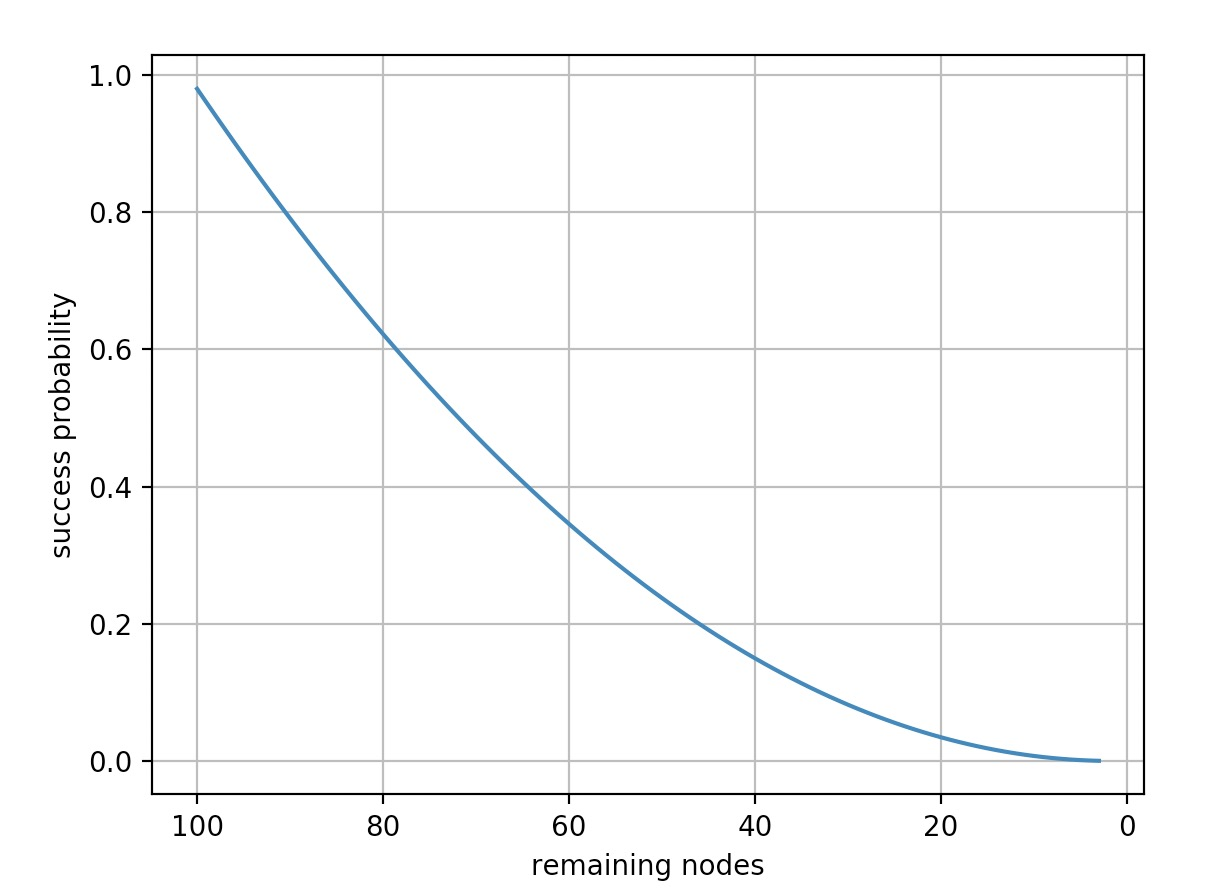
\includegraphics[scale=0.3]{images/min-cut-pic1.png}
    \caption{success probability vs. remaing nodes}
    \label{fig:fig1}
\end{figure}

Observing this image \ref{fig:fig1}, it's easy to sense that the curve declines more and more slowly as the number of remaining nodes decreases.
Thus, we can stop the contraction when the remaining nodes is ${\bf t}$, the procedure contraction can be adaptively changed.

This leaves us a question: What should ${\bf t}$ exactly be ?

In the original paper, Karger and Stein let $t = \lceil \frac{n}{\sqrt{2}} + 1 \rceil$.Because they hope to make equation \ref{eq: eq4}
return a probability $\geq \frac{1}{2}$.Denoting the set of contracted edges util remaining \textbf{t} nodes as \textbf{A}.
\begin{equation}\label{eq: eq5}
    \begin{aligned}
        Pr \bigg[ {\bf A} \cap {\bf C} = \emptyset \bigg] &\geq \prod_{i = 0}^{n - t - 1} (1 - \frac{2}{n - i}) \\
                                                          &= \frac{t (t - 1)}{n (n - 1)} \\
                                                          &\geq \frac{(t - 1)^2}{(n - 1)^2} \\
                                                          &\geq \frac{1}{2}                                       
    \end{aligned}
\end{equation}
Solve the equation above, we get $t = \lceil \frac{n}{\sqrt{2}} + 1 \rceil$.


\begin{algorithm}[h]
    \caption{Improved Contraction Algorithm: Contract({\bf G, t})}
    \begin{algorithmic}
        \Require graph {\bf G}, contraction stop threshold {\bf t}
        \Ensure sets of remaining edges

        \While{{\bf |V|} > {\bf t}}
            \State choose a uniform {\bf e} $\in$ {\bf E};
            \State contract({\bf e});
        \EndWhile
        \State \Return remaining edges in {\bf G}
    \end{algorithmic}
\end{algorithm}

As we use the improved contraction algorithm above, we can use accordingly modify the old Min-Cut algorithm to Fast-Cut algorithm:

\begin{algorithm}[h]
    \caption{Karger-Stein's Algorithm: Fast-Cut({\bf G})}
    \begin{algorithmic}[1]
        \Require graph {\bf G}, contraction stop threshold {\bf t}
        \Ensure number of remaining edges {\bf$|\hat{C}|$}
        \State set {\bf t} = $\lceil \frac{n}{\sqrt{2}} + 1 \rceil$
        \If{{\bf |V|} <= 6}
            \State perform min-cut algorithm by brute-force.
        \Else
            \State G1 = Contract({\bf G, t});
            \State G2 = Contract({\bf G, t});
        \EndIf
        \State \Return Min( {Fast-Cut(G1), Fast-Cut(G2)} )
    \end{algorithmic}
\end{algorithm}

What's the probability that Fast-Cut Algorithm return the correct {\bf C} ?
For graph {\bf G(V, E), |V| = n}, we define the probability as {\bf $P(n)$ }.As the 2 contractions are independent, we obtain:
\begin{equation}
    \begin{aligned}
        P(n) &= 1 - (1 - \frac{1}{2} P(\lceil \frac{n}{\sqrt{2}} + 1 \rceil))^2 \\
             &\geq 1 - \left( 1 - P(\lceil \frac{n}{\sqrt{2}} + 1 \rceil) + \frac{1}{4} P(\lceil \frac{n}{\sqrt{2}} + 1 \rceil)^2 \right) \\
             &= P(\lceil \frac{n}{\sqrt{2}} + 1 \rceil) - \frac{1}{4} P(\lceil \frac{n}{\sqrt{2}} + 1 \rceil)^2
    \end{aligned}
\end{equation}
By induction:
 \[
    P(\lceil \frac{n}{\sqrt{2}} + 1 \rceil) = \Omega(\frac{1}{\log{n}})
 \]

Fast-Cut algorithm is ensured to return the correct min-cut {\bf C} with probability {\bf at least} $ 1 - \frac{1}{n}$:
\begin{equation}
    \begin{aligned}
        1 - (1 - P(\lceil \frac{n}{\sqrt{2}} + 1 \rceil))^{\log^2{n}} &\geq 1 - (1 - \frac{1}{\log{n}})^{\log^2{n}} , \quad n \rightarrow \infty \\
                                                                      &= 1 - \bigg( \frac{1}{e} \bigg)^{log{n}} \\
                                                                      &= 1 - \frac{1}{n}
    \end{aligned}
\end{equation}


\subsection{Time complexity analysis of Fast-Cut Algorithm}
\begin{equation}
    \begin{aligned}
        T(n) &= 2 T(\lceil \frac{n}{\sqrt{2}} + 1 \rceil) + O(n^2)
    \end{aligned}
\end{equation}

Applying {\bf Master Theorem}, we can obtain that : 
\[
    T(n) = O(n^2 \log{n})
\]



\end{document}